\documentclass[tikz]{standalone}
\usepackage{pgfplots}
\pgfplotsset{compat=1.18}
\begin{document}
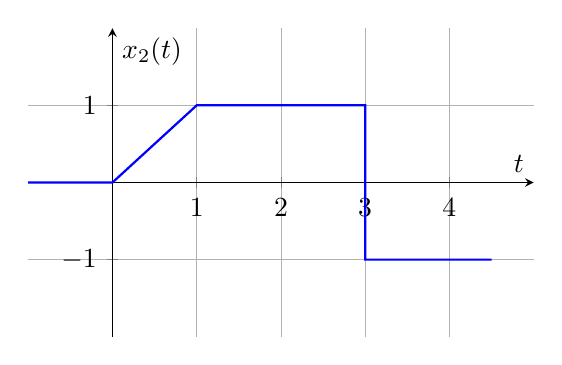
\begin{tikzpicture}
	\begin{axis}[
		width=8cm, height=5.5cm,
		axis lines=middle,
		xmin=-1, xmax=5, ymin=-2, ymax=2,
		xlabel={$t$}, ylabel={$x_2(t)$},
		grid=both,
		grid style={line width=.1pt, draw=gray!40},
		major grid style={line width=.2pt,draw=gray!60},
		xtick={0,1,2,3,4}, ytick={-1,0,1},
		samples=100
	]
	\addplot[thick, blue] coordinates {(-1,0) (0,0) (1,1) (3,1) (3,-1) (4.5,-1)};
	\end{axis}
\end{tikzpicture}
\end{document}
